\documentclass{exam}

\usepackage{amsmath}
\usepackage{amssymb}
\usepackage{amsthm}
\usepackage{graphicx}
\usepackage{esvect}
\usepackage{url} 

% Header and footer.
\pagestyle{headandfoot}
\runningheadrule
\runningfootrule
\runningheader{CS 440}{Refresher}{Fall 2021}
\runningfooter{}{Page \thepage\ of \numpages}{}
\firstpageheader{}{}{}

\qformat{{\large\bf Problem \thequestion. \thequestiontitle}\hfill}

\newcommand\mbf[1]{\ensuremath{\mathbf{#1}}}

\title{Refresher}
\author{CS 440 Computer Graphics\\Habib University}
\date{Fall 2021}

\begin{document}
\maketitle

\begin{questions}

  \titledquestion{Matrix Arithmetic}
  \begin{parts}
    \part Write down the 3x3 {\it identity matrix}.

    \part\label{transform} Given an $n\times n$ matrix, $A$, a vector, $x$, and the equation below
    \[ Ax = b, \]
    what are the dimensions of $x$ and $b$?

  \part Write down an expression for $x$ in (\ref{transform}).

  \part\label{eq} Write the following system of equations in matrix form.
    \begin{align*}
      2x + y - 2z	& =  3\\
      x - y - z & =	0\\
      x + y + 3z & = 12
    \end{align*}

    \part Solve the system of equations from (\ref{eq}).

    \part Find the transpose and inverse of the matrix
    \[
      \left(
        \begin{array}{ccc}
          1 & 2 & 1\\
          1 & 1 & 1\\
          2 & 1 & 1
        \end{array}
      \right)
    \].

  \end{parts}    

  \titledquestion{Vectors}
  Given the points $P(1,-2,0)$, $Q(3,1,4)$, and $R(0,-1,2)$, determine
  \begin{parts}
  \part the vectors $\vv{PQ}$ and $\vv{PR}$.

    \part\label{dot} the angle between the vectors $\vv{PQ}$ and $\vv{PR}$.

    \part a vector perpendicular to both $\vv{PQ}$ and $\vv{PR}$.

    \part the length of the projection of $\vv{PR}$ on $\vv{PQ}$.

    \part the unit vectors corresponding to $\vv{PQ}$ and $\vv{PR}$.

  \end{parts}

  \titledquestion{Geometry}
  Given the points $P(1,-2,0)$, $Q(3,1,4)$, and $R(0,-1,2)$, determine the {\it vector}, {\it scalar}, and {\it parametric} equations of the following.
  \begin{parts}
    \part the ray starting at $P$ and passing through $Q$.

    
  \part the circle with center at $P$ and passing through $Q$.

    
  \part the plane containing the points $P$, $Q$, and $R$.

  \end{parts}

\titledquestion{Linear Independence, Basis and Dimension}
  Given two vectors $\vv{v} = (1,2,0)$ and $\vv{w} = (2,3,0)$, find:
  \begin{parts}
  \part if $\vv{v}$ and $\vv{w}$ are linearly independent,

  \part if $\vv{v}$ and $\vv{w}$ are a basis for any space,

    
  \part the space $V$ which they span,

    
  \part the dimension of $V$.

  \end{parts}

\titledquestion{Trigonometry}
  In the right triangle below, the length of $AB$ is 13 units, and the length of $CB$ is 12 units.

    \centerline{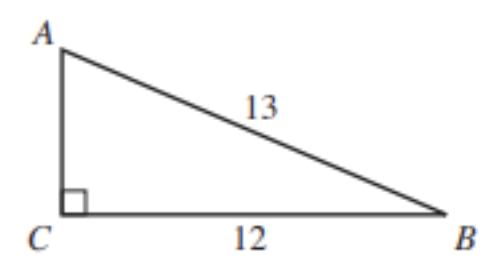
\includegraphics[width=300pt]{tri3}}
  \begin{parts}
  \part What is the tangent of $\angle A$?

  \part What is the sine of $\angle C$?

  \part What is the cosine of $\angle B$?

  \end{parts}

\titledquestion{Similar Triangles}
  Solve the following questions
  \begin{parts}
  \part A man, 6 feet tall, is walking away from a street light. If the length of the man’s shadow is 4 feet when he is 8 feet from the light, then how high is the light?

    \centerline{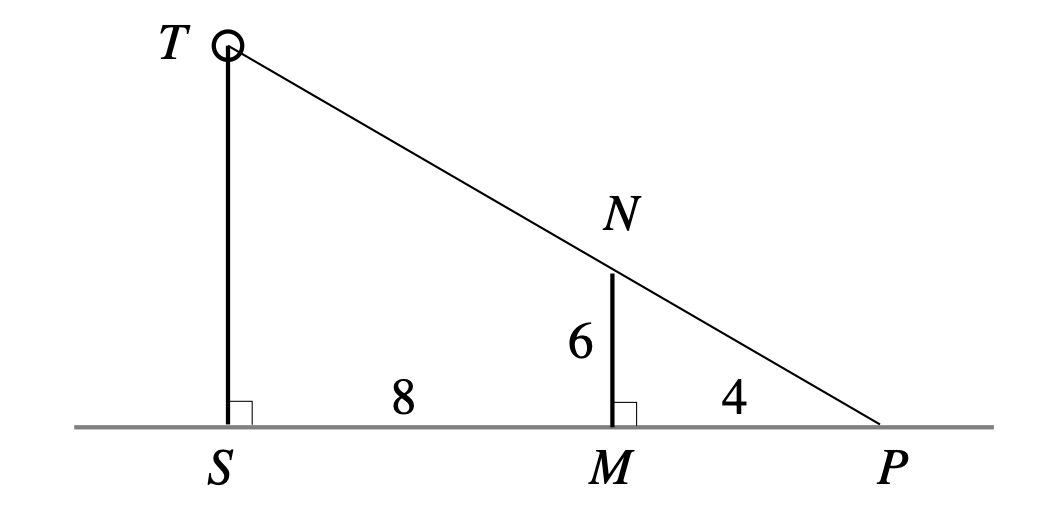
\includegraphics[width=300pt]{tri1}}

  \part The shadow of a flagpole has length 20 feet. At the same time, the length of the shadow of a yardstick is 6 inches. Find the height of the flagpole.

    \centerline{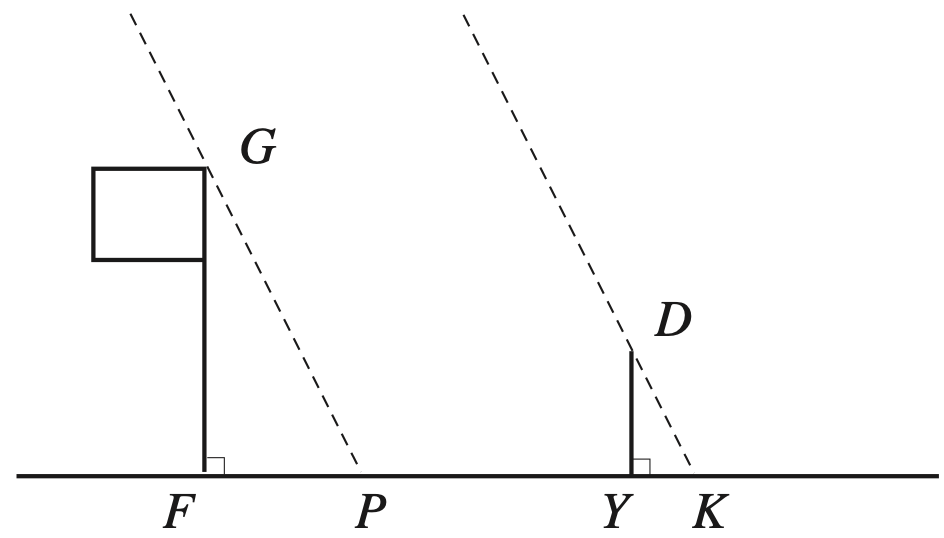
\includegraphics[width=300pt]{tri2}}    

  \end{parts}

\titledquestion{Linear Transformation}
  Solve the following.
  \begin{parts}
  \part Consider a vector $\vv{v}(0, 5)$, and find a transformation to rotate it $90^\circ$ anticlockwise.

  \part Consider a vector $\vv{v}(1, 3)$, and find a transformation to reflect it around y-axis.

  \end{parts}
  
\titledquestion{Vector Class}
  Implement a class, {\tt Vector}, in C++ to represent a 3D vector and define the following operations for it. Decide in each case whether the operation should be implemented as a method or an external function.
  \begin{parts}
    \part \underline{\tt dot}:  takes another {\tt Vector} object as a parameter and returns the dot product.
    \part \underline{\tt cross}: takes another {\tt Vector} object as a parameter and returns the cross product.
    \part \underline{\tt operator+}: takes another {\tt Vector} object as a parameter and returns the vector sum.
    \part \underline{\tt operator+=}: takes another {\tt Vector} object as a parameter and adds it to this {\tt Vector}.
    \part \underline{\tt operator-}: takes another {\tt Vector} object as a parameter and returns the vector difference.
    \part \underline{\tt operator-=}: takes another {\tt Vector} object as a parameter and subtracts it from the {\tt Vector}.
    \part \underline{\tt operator*}: takes a scalar as a parameter and returns the scaled vector. The operation must be commutative.
    \part \underline{\tt operator*=}: takes a scalar as a parameter and scales this {\tt Vector}.
    \part \underline{\tt norm}: returns the norm or magnitude of this {\tt Vector}.
    \part \underline{\tt normalize}: normalizes this {\tt Vector}.
    \part \underline{\tt operator-}: negates this {\tt Vector}.
  \end{parts}

\end{questions}

\section*{Credits}
Some of the questions have been adapted from:
\begin{itemize}
\item \url{https://math.dartmouth.edu/archive/m8s00/public_html/handouts/matrices3/node4.html}.
\item \url{http://tutorial.math.lamar.edu/Classes/CalcIII/EqnsOfPlanes.aspx}.
\item \url{http://srjcstaff.santarosa.edu/~jomartin/M27Folder/Handouts/SimilarTriangles.pdf}
\end{itemize}

\end{document}

%%% Local Variables:
%%% mode: latex
%%% TeX-master: t
%%% End:
